Ogni processo deve essere organizzato basandosi sul Ciclo di Deming.
\begin{itemize}
	\item \textbf{Pianificazione}: stabilire gli obiettivi e i processi necessari per fornire risultati in accordo con i risultati attesi;
	\item \textbf{Eseguire}: vengono implementate le attività secondo le linee definite durante la fase pianificazione;
	\item \textbf{Valutare}: viene verificato l'esito delle azioni di miglioramento rispetto alle attese;
	\item \textbf{Act}: azione per rendere definitivo e/o migliorare il processo. Richiede azioni correttive sulle differenze significative tra i risultati effettivi e previsti.
\end{itemize}
\begin{figure}[H]
\centering
	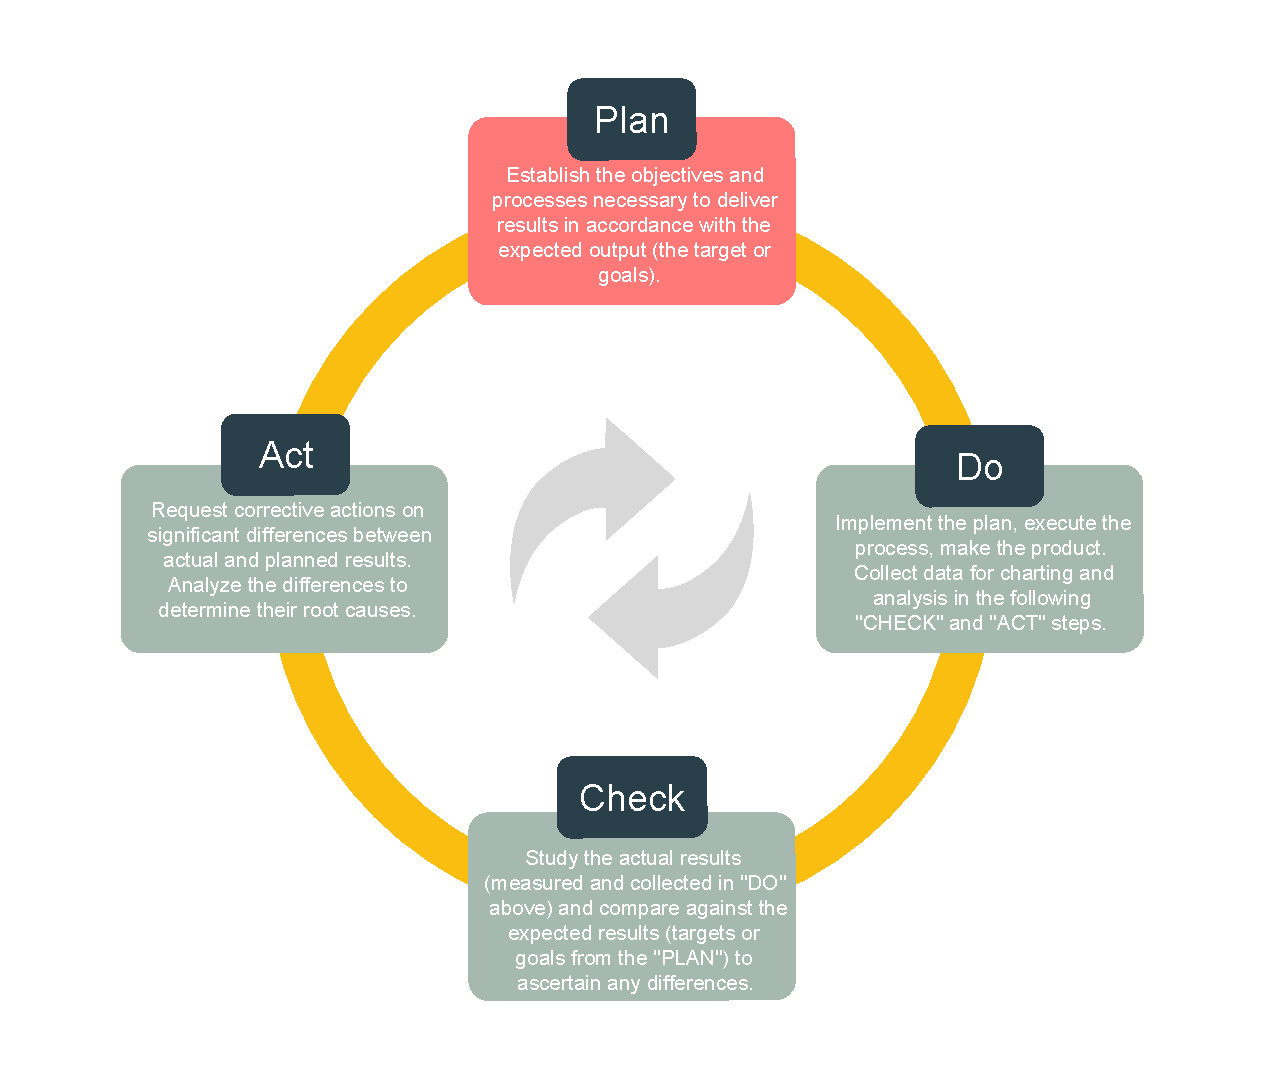
\includegraphics[scale=.7]{img/PDCA.pdf} 
	\caption{Ciclo di Deming}	
\end{figure}